\section{Verifikation und Validierung}
\label{sec:verifikationUndValidierung}

In diesem Abschnitt soll es um die Verifikation und Validierung der zuvor konzipierten und implementierten Applikationen gehen. Es wird also geprüft, ob die Software alle erwarteten Anforderungen vollständig erfüllt, den Bedürfnissen der Benutzer nachkommt und entsprechend der bestimmungsgemäßen Verwendung funktioniert.

\subsection{Einhaltung von Standards}
\label{subsec:standards}

Der erste und simpelste Punkt in diesem Kapitel soll eine Reflexion auf die Standards sein, welche für die Softwareentwicklung genutzt wurden. Neben der angemessenen Befolgung der Richtlinien des Europa Web Guide [\cite{guidelineWeb}], gilt es Standards wie den industriellen Cyber-Sicherheitsstandard IEC 62443 [\cite{IEC62443}] und Regulationen wie die europäische Regulation IEC 62443 [\cite{euDataProtectionRegulation}] zu befolgen. Dadurch, dass all diese Richtlinien, Standards und Regulationen bereits in die Konzeption der Applikationen integriert und bei der Implementierung befolgt wurden, muss nun keine Anpassung mehr vollzogen werden.

\subsection{Gleichzeitige Ausführung mehrerer Prozesse}
\label{subsec:gleichzeitigeAusführung}

Bei der aktuellen Architektur kann es zu Problemen führen, wenn mehrere Nutzer versuchen, gleichzeitig einen Prozess auszuführen oder wenn ein Nutzer sehr kurz nacheinander zwei langwierige Prozesse ausführt. In diesen Fällen würden die Befehle verschachtelt bei der API eingehen und damit auch verschachtelt an die PLC weitergeleitet werden, wo nicht mehr zwischen den beiden Prozessen unterschieden werden könnte. Falls die gleiche Anlage angesprochen wird, so kann es offensichtlich zu massiven Problemen führen, wenn zwei Prozesse gleichzeitig ausgeführt werden.\\
Um dieses Problem zu mildern, wurde die API in der Cloud um ein Nachrichten-System erweitert, welches sowohl benutzt werden kann, um alle Nutzer der Prozessplanungs-Seite darüber zu informieren, wenn und wann ein Benutzer einen Auftrag abgeschickt hat und wie lange dieser in etwa dauern wird, als auch um ein Warteschlangen-System einzurichten. Diese Warteschlange sorgt dann dafür, dass ein Nutzer einen Auftrag erst abschicken kann, wenn gerade kein anderer Auftrag ausgeführt wird.

In Grafik \ref{fig:eventLogAndQueue} sind die beiden Blöcke für das Ereignisprotokoll und die Warteschlange abgebildet. Diese Blöcke wurden unten auf die Prozessplanungs-Seite eingefügt, sodass sie von allen Nutzern während dem Benutzen des Prozess-Editors gesehen werden.
%
\begin{figure}[htbp]
	\centering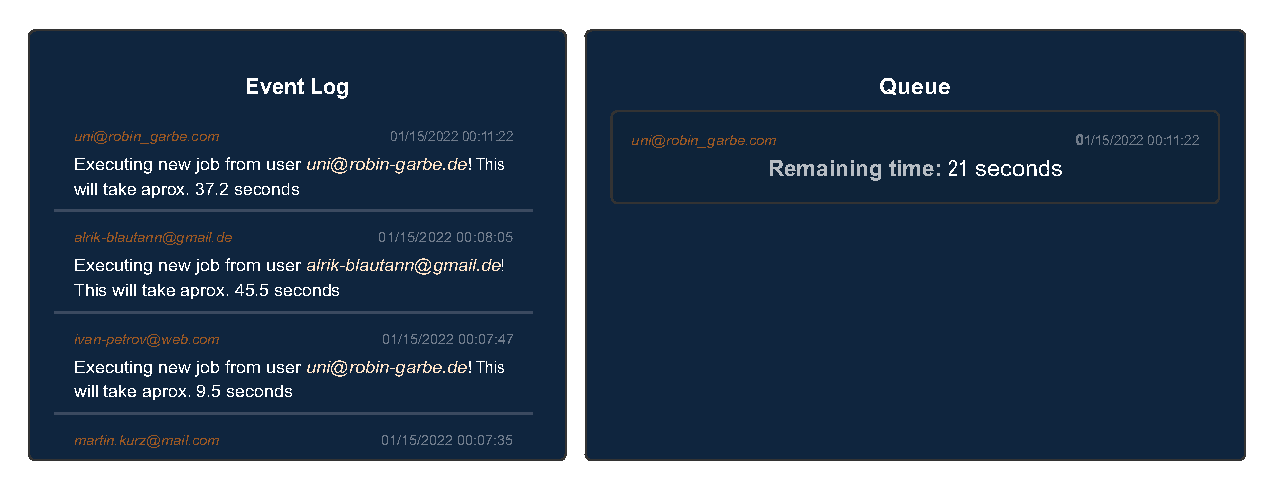
\includegraphics[width=1.0\textwidth]{images/06/EventLogAndQueue.eps}
    \caption{Ereignisprotokoll und Warteschlange}
    \label{fig:eventLogAndQueue}
\end{figure}

\subsection{Latenzen und Latenz-Varianzen}
\label{subsec:latenzen}

In Grafik \ref{fig:dtaProzessAblaufplan} wurde der Ablaufplan einer typischen Prozessplanung und -steuerung dargestellt. Wie dort zu sehen und in Kapitel \ref{sec:prozesssteuerung} beschrieben ist, wird für jede Aktivierung oder Deaktivierung eines Aktuators eine einzelne Anfrage an die Cloud und von dort and die entsprechende PLC gesendet. Dies macht es nötig, einen näheren Blick auf die Latenzen und vor allem die Latenz-Varianzen zu werfen, da eine Schwankung in den Ankunftszeiten der einzelnen Befehle den Programmfluss massiv beeinträchtigen könnte.\\
Um dieses Problem näher zu verdeutlichen, wird der in Grafik \ref{fig:PotenziellProblematischerProzess} dargestellte Prozess betrachtet. Bei diesem simplen Prozess wird zunächst ein Bauteil herausgegeben und daraufhin wird das Förderband aktiviert bevor es nach exakt 4,3 Sekunden wieder deaktiviert wird.
%
\begin{figure}[htbp]
	\centering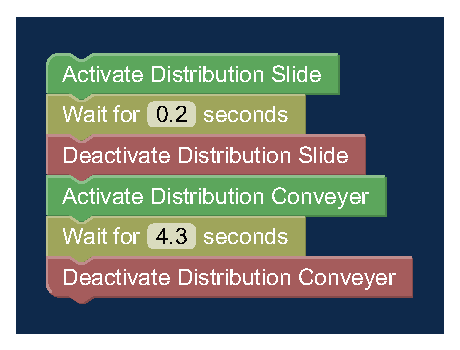
\includegraphics[width=0.5\textwidth]{images/06/LatenzVarianzProblem.eps}
    \caption{Potenziell problematischer Prozess}
    \label{fig:PotenziellProblematischerProzess}
\end{figure}

In diesem Beispiel sei die Dauer von 4,3 Sekunden dadurch relevant, weil das Bauteil nach exakt dieser Zeit unter einem weiteren Element wie einem RFID Lesegerät steht. Wenn das Förderband also nicht nach präzise dieser Dauer wieder deaktiviert wird, ist das Bauteil nicht genau unter dem Lesegerät und der Prozess kann nicht fortgesetzt werden. Die Latenz ist hier nicht hochgradig relevant, da es keine entscheidende Rolle spielt, nach wie vielen Millisekunden der Prozess gestartet wird. Die Latenz-Varianz ist allerdings von massiver Wichtigkeit, da eine hohe Varianz in diesem Beispiel bedeuten könnte, dass das Förderband kürzer oder länger aktiv ist. Ein Beispiel hierfür wäre, wenn der Aktivierungsbefehl für das Förderband nach 0,1 Sekunden bei der PLC eingeht, der Deaktivierungsbefehl aber 0,3 Sekunden benötigt; das Förderband wäre dann für 4,5 Sekunden aktiv.

Um zu überprüfen, ob die Latenz tatsächlich in einem problematischen Maß schwanken, wurden einige Testreihen am echten Gesamtsystem durchgeführt. Bei diesen drei Testreihen wurde je 20 Mal mit einer Verzögerung von je zehn Sekunden ein Aktuator über die API in der Cloud angesteuert. Es wurde die Differenzen der Zeitstempel zwischen dem Senden des Befehls und dessen Eingang auf der PLC protokolliert und nach den 20 Durchläufen wurde die höchste und niedrigste Zeitstempel-Differenz sowie die Differenz aus diesen beiden notiert. Es sei hier angemerkt, dass die Differenzen der Zeitstempel zwischen dem Senden und Empfangen nicht äquivalent sind zu der Latenz, da die internen Uhren der Testgeräte nicht exakt aufeinander abgestimmt sind.\\
In Tabelle \ref{tab:testreihenLatenzVarianz} stehen die Ergebnisse zu diesen drei Testläufen. Wie dort zu sehen ist, ist die Schwankung der Latenzen problematisch hoch. Die Latenz-Varianz hat bei diesen Testreihen etwa bei drei bis sechs Sekunden gelegen, was noch viel bedenklicher ist als zunächst vermutet. Bei einer Varianz von fünf Sekunden könnte es so passieren, dass im obigen Beispiel das Förderband statt 4,3 Sekunden sogar 9,3 Sekunden aktiviert sein könnte.
%
\bgroup
\def\arraystretch{1.5}
\vspace{5mm}\begin{table}[htbp]
    \centering
    \begin{tabularx}{156mm}{@{}p{23mm}*3{|>{\centering\arraybackslash}X}@{}}
        \rowcolor{dikblue} & \mbox{\color{white}\textbf{Minimale Zeist.-Diff.}} & \mbox{\color{white}\textbf{Maximale Zeist.-Diff.}} & \mbox{\color{white}\textbf{Varianz}}  \\
        Testreihe C1 & 3597897ms & 3603408ms & 5511ms \\ \hline
        Testreihe C2 & 3597918ms & 3601218ms & 3300ms \\ \hline
        Testreihe C3 & 3597972ms & 3600962ms & 2990ms
    \end{tabularx}
    \caption{Testreihen zur Messung der Latenz-Varianz über die Cloud}
    \label{tab:testreihenLatenzVarianz}
\end{table}
\egroup

Um dieses Problem zu lösen, könnte der Steuerungsablauf so angepasst werden, dass die Befehle nicht einzeln vom Browser gesendet werden, sondern dass der Browser den gesamten Prozess in einer Anfrage sendet. Die Applikation in der Cloud würde den Prozess dann an einen Computer – welcher sich im gleichen lokalen Netz wie die anzusteuernde PLC befindet – senden. Dieser Computer würde den erhaltenen Prozess dann parsen und ausführen, wobei er die einzelnen Befehle sowohl als Update an die Datenbank weitergibt, sodass diese stets ein Abbild des aktuellen Zustandes hat, als auch an die PLC sendet. Die Latenz-Varianzen bei einer Übertragung im lokalen Netz an die PLC sind verschwindend gering. Um dies zu zeigen, wurden drei weitere Testreihen durchgeführt, bei welchen je 100 Befehle in einem zufällig gewählten Abstand von 1 bis 2 Sekunden gesendet werden. Wie im letzten Testlauf wurden die Ergebnisse notiert und sind in Tabelle \ref{tab:testreihenLatenzVarianzLokal} aufgeführt. Die Latenz-Varianzen sind hier wie vermutet mit unter 20 Millisekunden vernachlässigbar niedrig.
%
\bgroup
\def\arraystretch{1.5}
\vspace{5mm}\begin{table}[htbp]
    \centering
    \begin{tabularx}{156mm}{@{}p{23mm}*3{|>{\centering\arraybackslash}X}@{}}
        \rowcolor{dikblue} & \mbox{\color{white}\textbf{Minimale Zeist.-Diff.}} & \mbox{\color{white}\textbf{Maximale Zeist.-Diff.}} & \mbox{\color{white}\textbf{Varianz}}  \\
        Testreihe L1 & 3558532ms & 3558547ms & 15ms \\ \hline
        Testreihe L2 & 3558538ms & 3558542ms & 4ms \\ \hline
        Testreihe L3 & 3558539ms & 3558551ms & 12ms
    \end{tabularx}
    \caption{Testreihen zur Messung der Latenz-Varianz über das lokale Netzwerk}
    \label{tab:testreihenLatenzVarianzLokal}
\end{table}
\egroup

Die beschriebene neue Kommunikations-Infrastruktur ist in Grafik \ref{fig:verbesserteKommunikationsInfrastruktur} abgebildet. Der wesentliche Unterschied zur vorherigen Infrastruktur (abgebildet in Grafik \ref{fig:dtaInfrastrukturÜbersicht}) ist das Hinzunehmen eines Computers im lokalen Netz der Anlage. Dies ist jedoch wenig problematisch, da ein solcher Computer in der aktuell eingesetzten Infrastruktur ohnehin bereits eingesetzt wird, um den Live-Videostream der Anlage aufzunehmen und zu senden.
%
\begin{figure}[htbp]
	\centering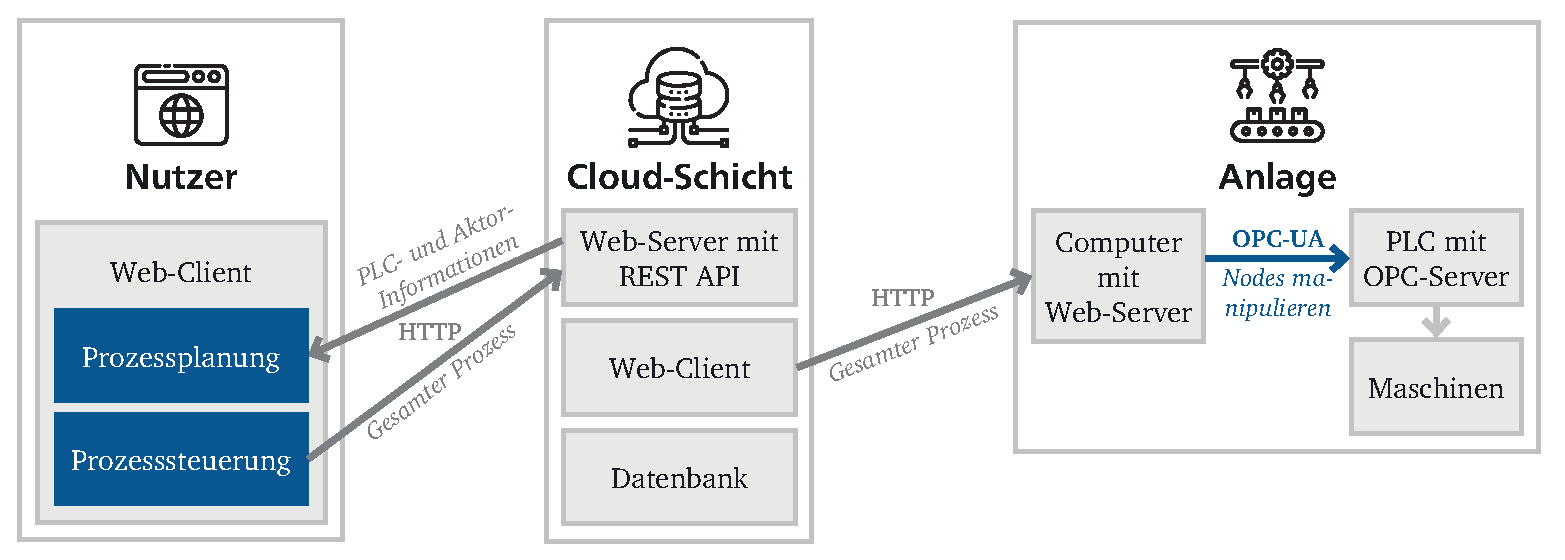
\includegraphics[width=1.0\textwidth]{images/06/verbesserteKommunikationsInfrastruktur.eps}
    \caption{Verbesserte Kommunikations-Infrastruktur}
    \label{fig:verbesserteKommunikationsInfrastruktur}
\end{figure}

\subsection{Tests}
\label{subsec:tests}

Da die aktuelle Webseite der Digital Twin Academy aufgrund ihrer Authentifizierung und ihres ständig ändernden Aufbaus ein automatisiertes Testen praktisch unmöglich macht, wurden manuelle Tests verwendet. Im Folgenden werden die getesteten Aspekte der Prozessplanungs und -steuerungs sowie der Produktionsplanungs-Applikation aufgeführt:

\subsection*{Endbenutzergesteuerte Prozessplanung und -steuerung}

\begin{itemize}
    \item Kompatibilität mit den in Kapitel \ref{subsec:prozessplanung_konzeption} spezifizierten Browsern wurde getestet
    \item Uneingeschränkte Benutzbarkeit in diesen Browsern wurde überprüft
    \item Korrektheit der gesendeten API-Anfragen wurde sichergestellt
    \begin{itemize}
        \item Sowohl bei der Generierung des Editors als auch bei der Ausführung eines Prozesses sind alle Aufrufe der API an eine korrekte Adresse, mit der korrekten Methode und mit einem eventuellen Rückgabewert wird korrekt umgegangen
    \end{itemize}
    \item Fehlerfälle wie etwa eine Benutzung ohne gültige Autorisierung wurden überprüft
    \item Angriffsmöglichkeiten wie das Senden von ungültigen oder zu vielen Anfragen wurden erprobt
\end{itemize}

\subsection*{Automatisierte und anpassbare Produktionsplanung}

Da es sich bei dieser Applikation lediglich um eine konzeptuelle Umsetzung in Form einer Benutzeroberfläche handelt, beschränken sich die überprüften Punkte auf die Kompatibilität und Benutzbarkeit in verschiedenen Browsern.

\subsection{Simulation}
\label{subsec:simulation}

Statt einen Prozess direkt an eine Anlage zu senden, sollte es möglich sein, ihn stattdessen an eine Simulation zu übergeben. Der Zustand dieser Simulation würde dann in Echtzeit als 3D Animation mittels Unity-Applet angezeigt werden, ähnlich wie auch der Zustand der echten Anlage in nahezu Echtzeit als Videostream angezeigt wird. Eine grundlegende Virtualisierung der Anlage sowie eine grobe Interaktion mit dieser Simulation besteht zwar bereits, allerdings ist dieses System zum Zeitpunkt dieser Arbeit noch bei Weitem nicht ausgereift genug, um es als Simulationsumgebung nutzen zu können. Es wurden allerdings die nötigen Weichen in der Prozesssteuerung angelegt, um eine solche Simulation in Zukunft problemlos zu ermöglichen, sobald eine Umgebung dafür besteht.

\subsection*{Ergebnisse der Verifikation und Validierung}
\label{subsec:ergebnisse}

Als Ergebnis der oben beschriebenen Punkte wurde die Funktion, Korrektheit und Sicherheit der Applikationen für den Kontext als konzeptuelle Umsetzung zufriedenstellend verifiziert und validiert. Mit Blick auf die Gesamtarchitektur sind weitere Schritte in den Bereichen der Cyber-Sicherheit möglich und für eine industrielle Anwendung nötig, jedoch liegen die hier zu verändernden Aspekte außerhalb des Umfangs dieser Arbeit und sind primär bei der Weiterentwicklung des C\# Programmes und spezifischer der REST API zu finden.